

\documentclass{article}

\usepackage{lipsum} % Package to generate dummy text throughout this template

\usepackage[sc]{mathpazo} % Use the Palatino font
\usepackage[T1]{fontenc} % Use 8-bit encoding that has 256 glyphs
\linespread{1.2} % Line spacing - Palatino needs more space between lines
\usepackage{microtype} % Slightly tweak font spacing for aesthetics

\usepackage[hmarginratio=1:1,top=32mm,columnsep=20pt]{geometry} % Document margins
\usepackage{multicol} % Used for the two-column layout of the document
\usepackage[hang, small,labelfont=bf,up,textfont=it,up]{caption} % Custom captions under/above floats in tables or figures
\usepackage{booktabs} % Horizontal rules in tables
\usepackage{float} % Required for tables and figures in the multi-column environment - they need to be placed in specific locations with the [H] (e.g. \begin{table}[H])
\usepackage{hyperref} % For hyperlinks in the PDF

\usepackage{lettrine} % The lettrine is the first enlarged letter at the beginning of the text
\usepackage{paralist} % Used for the compactitem environment which makes bullet points with less space between them
\usepackage{graphicx}
\usepackage{graphics}

\usepackage{abstract} % Allows abstract customization
\renewcommand{\abstractnamefont}{\normalfont\bfseries} % Set the "Abstract" text to bold
\renewcommand{\abstracttextfont}{\normalfont\small\itshape} % Set the abstract itself to small italic text

\usepackage{titlesec} % Allows customization of titles
\renewcommand\thesection{\Roman{section}} % Roman numerals for the sections
\renewcommand\thesubsection{\Roman{subsection}} % Roman numerals for subsections
\titleformat{\section}[block]{\large\scshape\centering}{\thesection.}{1em}{} % Change the look of the section titles
\titleformat{\subsection}[block]{\large}{\thesubsection.}{1em}{} % Change the look of the section titles

\usepackage{fancyhdr} % Headers and footers
\pagestyle{fancy} % All pages have headers and footers
\fancyhead{} % Blank out the default header
\fancyfoot{} % Blank out the default footer
\fancyhead[C]{Wireless Communications $\bullet$ September 2015} % Custom header text
\fancyfoot[RO,LE]{\thepage} % Custom footer text

%----------------------------------------------------------------------------------------
%	TITLE SECTION
%----------------------------------------------------------------------------------------

\title{\vspace{-15mm}\fontsize{24pt}{10pt}\selectfont\textbf{IT 601 ASSIGNMENT 1}} % Article title

\author{
\large
\textsc{Wilson Chanhemo, Noel Chintelele, Said A. Kombo, Noel Chintelele}\thanks{Wireless Communications}\\[2mm] % Your name
\normalsize University of Dodoma \\ % Your institution
\vspace{-5mm}
}
\date{}

%----------------------------------------------------------------------------------------

\begin{document}

\maketitle % Insert title

\thispagestyle{fancy} % All pages have headers and footers

%----------------------------------------------------------------------------------------
%	ARTICLE CONTENTS
%----------------------------------------------------------------------------------------


\section{question}
Simulate and plot the capacity of a Rayleigh fading channel vs. the average SNR for the following cases:\\
a)	CSI is known at both the transmitter and the receiver,\\
b)	CSI is known at the receiver only,\\
c)	Channel inversion power control is used,\\
d)	Maximum outage capacity,\\
e)	AWGN channel capacity with the same average SNR as the Rayleigh channel.\\

Simulate for average transmits SNR $\gamma=P/\sigma^2$   in the range 0 to 30dB in steps of 5 dB and generate 10,000 of channel realizations for each value of SNR. To generate Rayleigh fading channel vector of length N, use the following Matlab code  h=(randn(1,N)+irandn(1,N))/$\sqrt{2}$

%------------------------------------------------

\section{Transmitter and Receiver CSI}

For CSI at both the transmitter and the receiver, the following capacity formula is used\\
$C=\sum _{{\gamma }_{0}}^{\infty }B{\mathrm{log}}_{2}\left(\frac{{\gamma }_{i}}{{\partial }_{0}}\right)p\left({\gamma }_{i}\right)$\\ But for simulation purposes, values of h are used to generate the Rayleigh channel behavior, so this capacity can be equivalently represented as\\
$C=E\left[\Sigma B{\mathrm{log}}_{2}\left[\frac{P{\left|h\right|}^{2}}{{\gamma}_{0}\sigma^2}\right]\right]$\\ The corresponding matlab code is shown below\\
%New line for matlab code
\% RAYLEIGH CHANEL CAPACITY WITH \\RECEIVER AND TRANSMITER CSI
snrdB=0:5:30; %Range of SNRs to simulate\\
$h=(randn(1,10000) + 1i*randn(1,10000))/sqrt(2);$ %Rayleigh flat channel \\ 
sigmz=1; \%Noise power - assumed to be unity\\
SNRo=1; \% Assume minimum SRN Equal to unity\\
$snr = 10.^(snrdB/10); $\%SNRs in linear scale%\\
$P=(sigmz^2)*snr./(mean(abs(h).^2));$\\ %Calculate corresponding values for P\\
$Cerg = mean((log2(((abs(h).^2).')*P)));$\\
plot(snrdB,Cerg,'b');grid on;\\
legend('Chanel Capacity');\\
title('Ergodic capacity with Rx and Tx CSI SNRo normalized to 1');\\
xlabel('SNR (dB)');ylabel('Capacity (bps/Hz)');\\

%Simulation results
\begin{figure}
\centering
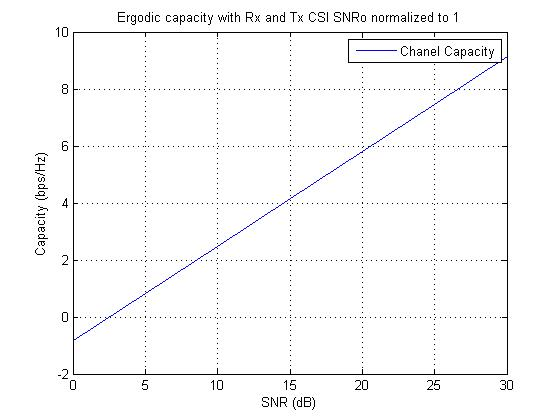
\includegraphics[width=1\linewidth]{RxTxCSI}
\caption{}
\label{fig:RxTxCSI}
\end{figure}
\section{Receiver CSI}
Using the same concept as in (a), Capacity for this channel is given by the expression\\ $C=\sum _{\stackrel{.}{i}}^{n}B{\mathrm{log}}_{2}\left(1+{\gamma}_{i}\right)p\left({\gamma}_{i}\right)$ \\For a Rayleigh channel by h, this can be written as\\ $c=E\left(\sum B{\mathrm{log}}_{2}\left(1+\frac{p{\left|h\right|}^{2}}{{b}^{2}}\right)\right)$. The corresponding matlab code is shown below. Resulting simulation is shown in Figure 2.\\

\% RAYLEIGH CHANEL CAPACITY WITH RECEIVER CSI
snrdB=0:5:30; \%Range of SNRs to simulate\\

$h= (randn(1,10000) + 1i*randn(1,10000) )/\sqrt(2);$ \%Rayleigh flat channel\\
sigmaz=1;\ %Noise power - assumed to be unity\\
$snr = 10.^(snrdB/10);$ \%SNRs in linear scale\\
$P=(sigmaz^2)*snr./(mean(abs(h).^2))$; \%Calculate corresponding values for P\\
$Cerg = mean((log2(1+ ((abs(h).^2).')*P/(sigmaz^2))));$ \%ergodic capacity for Fading channel \\
plot(snrdB,Cerg,'r'); grid on;\\
legend('Fading channel Ergodic capacity');\\
title('Ergodic capacity Receiver CSI');\\
xlabel('SNR (dB)');ylabel('Capacity (bps/Hz)');\\
%Simulation Results
\begin{figure}
	\centering
	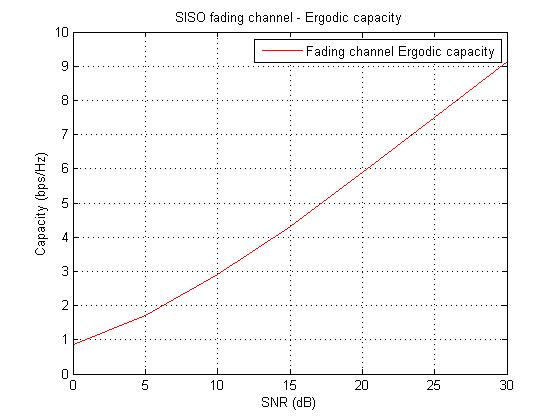
\includegraphics[width=1\linewidth]{RECEIVER_CSI}
	\caption{Capacity with Receiver CSI}
	\label{fig:RECEIVER_CSI}
\end{figure}

\section{Capacity with channel inversion }
With channel inversion, capacity is given as\\ $C=B{\mathrm{log}}_{2}\left(1+\frac{1}{E\left(\frac{1}{\gamma}\right)}\right)$.\\ With h effects, this capacity is also represented as\\ $C=B{\mathrm{log}}_{2}\left(1+\frac{1}{E\left(\frac{{\delta }^{2}}{P{\left|h\right|}^{2}}\right)}\right)$\\
% Matlab code
Matlab code is then shown here\\
snrdB=0:5:30; \%Range of SNRs to simulate\\
$h= (randn(1,10000) + 1i*randn(1,10000) )/sqrt(2);$ %Rayleigh flat channel\\
$sigmaz=1; \%Noise power - assumed to be unity\\
snr = 10.^(snrdB/10); \%SNRs in linear scale\\
P=(sigmaz^2)*snr./(mean(abs(h).^2));$ \%Calculate corresponding values for P\\

$Cinv= log2(1+ 1./(mean(1./(abs(h).^2)).*P/(sigmaz^2)));$ \%Capacity with chanel inversion\\
plot(snrdB,Cinv,'b');grid on;\\

legend('Chanel Invesion Capacity');\\
title('Capacity with chanel inversion');\\
xlabel('SNR (dB)');ylabel('Capacity (bps/Hz)');\\

%Ploting the simulation
Results of this simulation code is shown in Figure 3\\
\begin{figure}
	\centering
	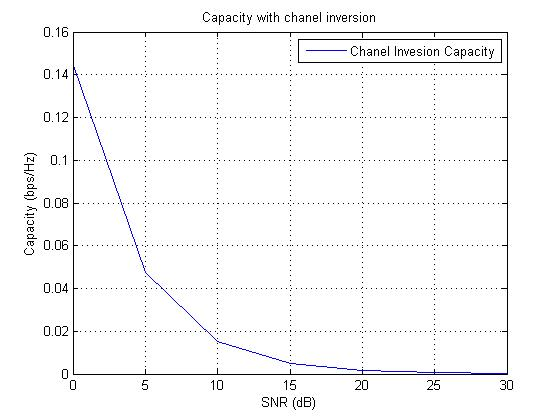
\includegraphics[width=1\linewidth]{Chanel_inv}
	\caption{Capacity with Channel Inversion}
	\label{fig:Chanel_inv}
\end{figure}

\section{Maximum Outage }
Maximum outage is channel inversion with cut off signal-to-noise ratio. In this case the capacity is that of channel inversion scaled down by probability of outage value. In this case if we take as 99\% of outage, capacity is thus given as \\
$C=B{\mathrm{log}}_{2}\left(1+\frac{1}{E\left(\frac{{\delta }^{2}}{P{\left|h\right|}^{2}}\right)}\right)*0.11$\\
The corresponding matlab code and simulation is shown in Figure 4.\\

snrdB=0:5:30; %Range of SNRs to simulate\\
$h= (randn(1,10000) + 1i*randn(1,10000) )/\sqrt(2)$; \%Rayleigh flat channel\\
sigmaz=1; \%Noise power - assumed to be unity\\
$snr = 10.^(snrdB/10);$ \%SNRs in linear scale\\
$P=(sigmaz^2)*snr./(mean(abs(h).^2));$ \%Calculate corresponding values for P\\
$Cout= log2(1+ 1./(mean(1./(abs(h).^2)).*P/(sigmaz^2)))*0.01$;\\ \%Capacity with maximum outage of 99\%\\
plot(snrdB,Cout,'r');grid on;\\
legend('Max Outage');\\
title('channel at maximum outage');\\
xlabel('SNR (dB)');ylabel('Capacity (bps/Hz)');\\
\\
%Ploting
\begin{figure}
	\centering
	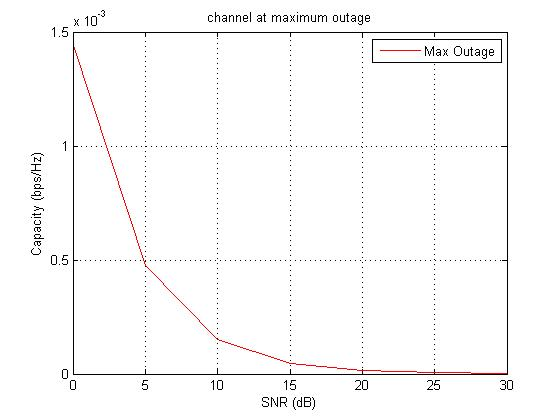
\includegraphics[width=1\linewidth]{Maxi_outage}
	\caption{Channel Capacity at 99\% Outage}
	\label{fig:Maxi_outage}
\end{figure}

\section{AWGN channel capacity with the same average SNR as the Rayleigh channel}
For AWGN channel with same average SNR as Rayleigh channel, capacity is given as \\
$C=B{\mathrm{log}}_{2}\left(1+E\left(\frac{P{\left|h\right|}^{2}}{{\delta }^{2}}\right)\right)$\\
This capacity is simulated by the following code.\\
snrdB=0:5:30; \%Range of SNRs to simulate \\
$h= (randn(1,100) + 1i*randn(1,100) )/sqrt(2)$; \%Rayleigh flat channel\\
sigmaz=1; \%Noise power - assumed to be unity\\
$snr = 10.^(snrdB/10); \%SNRs in linear scale\\
P=(sigmaz^2)*snr./(mean(abs(h).^2))$; \%Calculate corresponding values for P \\
$Cergawgn= (log2(1+ mean((abs(h).^2)).*P/(sigmaz^2)))$; \%AWGN channel capacity (Bound)\\
$Cerg = mean((log2(1+ ((abs(h).^2).')*P/(sigmaz^2))))$; \%ergodic capacity for Fading channel \\
plot(snrdB,Cergawgn,'b'); hold on;\\
plot(snrdB,Cerg,'r'); grid on;\\
legend('AWGN channel capacity','Fading channel Ergodic capacity');\\
title('SISO fading channel - Ergodic capacity');\\
xlabel('SNR (dB)');ylabel('Capacity (bps/Hz)');\\
//
%Simulation Results
\begin{figure}
	\centering
	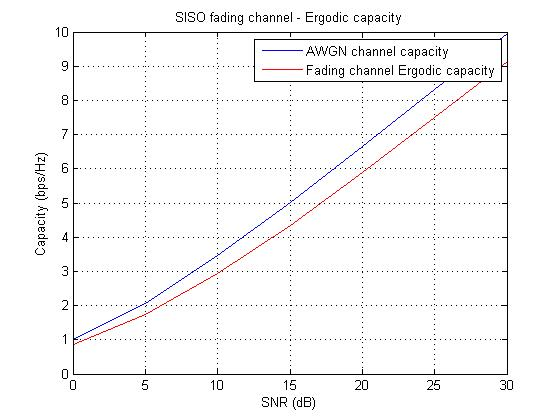
\includegraphics[width=1\linewidth]{AWGNasrayleigh}
	\caption{AWGN capacity with average SNR as Rayleigh channel}
	\label{fig:AWGNasrayleigh}
\end{figure}

\section{Results and Conclusion}
From the simulations above, we can note the following observation;
•	For receiver and transmitter CSI, capacity of the channel increase linearly with increase in SNR at normalized cut off SNR equal to a unit (Figure 1)\\
•	For receiver CSI, capacity of a fading channel exponentially increase with increase in SNR (Figure 2)\\
•	With channel inversion, capacity decay exponentially with increase in SNR (Figure 3)\\
•	With maximum outage, the decay is the same as for channel inversion but with capacity scaled by (1-Pout), where Pout is the outage probability (Figure 4)\\
•	With AWGN channel containing average SNR as that of Rayleigh fading channel, capacity has exponential growth but is more less than that of Rayleigh channel (Figure 5)\\



\end{document}
